\documentclass[11pt,a4paper]{article}

\usepackage[T1]{fontenc}
\usepackage[utf8]{inputenc}
\usepackage{lmodern}
\usepackage[margin=2.2cm]{geometry}
\usepackage{amsmath,amssymb}
\usepackage{graphicx}
\usepackage{booktabs}
\usepackage{array}
\usepackage{xcolor}
\usepackage{caption}
\usepackage{enumitem}
\usepackage{fancyhdr}
\usepackage{longtable}
\usepackage[hidelinks]{hyperref}

\definecolor{fnoblue}{HTML}{3573B9}
\definecolor{donrose}{HTML}{B03A5B}
\definecolor{pfnogold}{HTML}{C98A00}
\definecolor{ink}{HTML}{222222}
\definecolor{muted}{HTML}{5B5B5B}
\definecolor{rule}{HTML}{D8D8D8}
\definecolor{codebg}{HTML}{F7F7F5}

\hypersetup{colorlinks=true,linkcolor=fnoblue,urlcolor=fnoblue}
\captionsetup{font=small,labelfont={bf,small}}

\pagestyle{fancy}
\fancyhf{}
\lhead{\small\color{muted}SciML Project --- overview}
\rhead{\small\color{muted}\thepage}
\renewcommand{\headrulewidth}{0.4pt}

\newcommand{\relL}{relative $L_2$}
\newcommand{\bk}{\discretionary{}{}{}}
\emergencystretch=3em
\hbadness=10000

\setlength{\parskip}{2pt}

\title{\vspace{-1.4cm}\bfseries What this project does\\[2mm]
\large Two families of neural PDE solver on the 1D elastic wave equation}
\author{\normalsize SciML Project --- wave equation}
\date{\normalsize\today}

\begin{document}
\maketitle
\thispagestyle{fancy}

\noindent\fcolorbox{rule}{codebg}{%
\begin{minipage}{0.977\textwidth}
\small
\textbf{Summary.} One physics problem --- the 1D elastic wave equation in
heterogeneous media --- is attacked with two unrelated families of neural
solver, both measured against the same finite-difference reference.
\emph{Arm~A} trains physics-informed coordinate networks (seven architectures,
two compute backends, a 528-run sweep) that learn $(x,t)\mapsto u(x,t)$ for a
single material from the PDE residual alone. \emph{Arm~B} trains neural
operators (FNO, DeepONet, PFNO) that learn the map from an entire material
profile to the complete wavefield, supervised on FD solutions, and generalize to
media never seen in training. Arm~B is where the measured results are: after
diagnosing an under-specified training set, validation error falls from
$81.9\%$ to $\mathbf{1.96\%}$ (FNO), $94.8\%$ to $\mathbf{4.03\%}$ (PFNO) and
$97.3\%$ to $\mathbf{24.57\%}$ (DeepONet) on synthetic media, and the same
architectural ranking survives on three published geological velocity models.
Along the way: an unconverged reference target was found to have flattered one
architecture by ten points, the worst model was found to score the best
boundary residual, and adding physics losses was found to help a model that
already fits while pushing an underfitting one further toward collapse.
This document is the map --- what exists, what was found, and where it lives.
\end{minipage}}

\vspace{4mm}
{\small\tableofcontents}
\clearpage

%==============================================================
\section{The two arms}

The governing equation is
\begin{equation}
\rho(x)\,u_{tt} \;=\; \frac{\partial}{\partial x}\!\left[E(x)\,u_x\right],
\qquad x\in[-1,1],\quad t\in[0,1].
\end{equation}

The two arms share nothing but this equation and the reference solver.

\begin{center}
\small
\begin{tabular}{@{}>{\raggedright\arraybackslash}p{2.6cm}>{\raggedright\arraybackslash}p{6.0cm}>{\raggedright\arraybackslash}p{6.0cm}@{}}
\toprule
 & \textbf{Arm A --- coordinate networks} & \textbf{Arm B --- neural operators}\\
\midrule
learns & $(x,t)\mapsto u(x,t)$ for \emph{one} material
       & $[E(x),\rho(x),\dots]\mapsto u(x,t)$ for \emph{any} material\\[2pt]
supervision & PDE residual (no solution data) & FD solutions (supervised)\\[2pt]
cost model & retrain per problem & train once, infer in one forward pass\\[2pt]
question & which architecture / optimizer / weighting trains a PINN best?
         & which operator architecture generalizes to unseen media?\\[2pt]
models & VanillaPINN, FourierFeaturePINN, PirateNet, WavKAN, KAN,
         ChebyshevKAN, FourierWavKAN
       & FNO, DeepONet, PFNO\\[2pt]
status & infrastructure complete; 528-run sweep runs on Sherlock
       & \textbf{run, measured, documented}\\
\bottomrule
\end{tabular}
\end{center}

Arm~B is where the results are. Its full write-up --- physics, architectures,
diagnosis, per-arm results, visualization rationale, limitations --- is
\texttt{docs/operator\_simulations.\bk pdf}. What follows is the map.

%==============================================================
\section{The shared foundation}

\paragraph{The equation is solved in conservative form.} Expanding gives
$\rho u_{tt}=E u_{xx}+E_x u_x$, so the naive $u_{tt}=c(x)^2u_{xx}$ drops the
$E_x u_x$ term --- exactly the term that produces correct reflection and
transmission amplitudes at a material interface. Everything in the repository
uses the conservative form.

\paragraph{The FD reference} (\texttt{wave/fd\_solver.py}) is an explicit
second-order leapfrog scheme in flux form. Two details are load-bearing, and
both were arrived at by fixing a failure:

\begin{itemize}[leftmargin=*,itemsep=2pt]
\item \textbf{Harmonic-mean interface stiffness}
$E_{i+1/2}=2E_iE_{i+1}/(E_i+E_{i+1})$, which preserves transmission and
reflection across a jump in $E$.
\item \textbf{Mur discretization} of the absorbing boundaries,
$\beta=(c\,\Delta t-\Delta x)/(c\,\Delta t+\Delta x)$. The apparently natural
centred-time / one-sided-space ABC is \emph{unconditionally unstable}.
\end{itemize}

\paragraph{The reference has to be grid-converged.} This was not true initially,
and it turned out to matter (\S\ref{sec:converged}). Measured against a
\texttt{refine=32} solve:

\begin{center}
\small
\begin{tabular}{lrrr}
\toprule
\textbf{refine} & \textbf{FD grid} & \textbf{\relL{} vs converged} & \textbf{cost / 512 samples}\\
\midrule
1  & 64   & $13.35\%$ & 1.8 s\\
4  & 253  & $1.14\%$  & 8.9 s\\
\textbf{8} & \textbf{505} & $\mathbf{0.32\%}$ & \textbf{22 s}\\
16 & 1009 & $0.08\%$  & 41 s\\
\bottomrule
\end{tabular}
\end{center}

The problem definition --- initial condition, material sampler, refined solve,
input-channel layout --- lives in \texttt{wave/wave\_problem.py}, deliberately
torch-free so that dataset generation runs on machines with no GPU stack.

%==============================================================
\section{Arm A --- PINN / KAN coordinate networks}

Seven architectures compared on three canonical materials (Homogeneous,
TwoLayer, MultiLayer), trained purely on PDE residuals.

\subsection{Architectures}

\begin{center}
\small
\begin{tabular}{@{}l>{\raggedright\arraybackslash}p{10.2cm}@{}}
\toprule
\textbf{Model} & \textbf{Key idea}\\
\midrule
\texttt{VanillaPINN}        & MLP, Tanh $+$ Xavier initialization\\
\texttt{FourierFeaturePINN} & trainable random Fourier embedding $\to$ MLP\\
\texttt{PirateNet}          & fixed Fourier embedding $\to$ RWF layers $\to$ residual blocks ($\alpha$ init $0$)\\
\texttt{WavKAN}             & wavelet KAN (Mexican Hat / Morlet / DoG / Meyer / Shannon)\\
\texttt{KAN}                & spline KAN via \texttt{pykan} / \texttt{jaxkan}\\
\texttt{ChebyshevKAN}       & cPIKAN --- tanh-squashed inputs, Chebyshev recurrence per edge\\
\texttt{FourierWavKAN}      & Fourier embedding $\to$ WavKAN trunk (spectral-bias fix for sharp interfaces)\\
\bottomrule
\end{tabular}
\end{center}

\textbf{Both backends implement all seven.} PyTorch is the original; JAX/Equinox
is a parallel reimplementation (\texttt{src/*\_jax.py}) and is now the default.
The JAX path computes the PDE residual with
\texttt{jax.grad(jax.grad($\cdot$))} $+$ \texttt{vmap} rather than
reverse-over-reverse autograd, and uses \texttt{segment\_sum} for causal
chunking instead of a Python loop.

\subsection{Training machinery}

All of the following is implemented and switchable per run:

\begin{itemize}[leftmargin=*,itemsep=3pt]
\item \textbf{Two-phase schedule} --- Adam (15\,000 steps) then L-BFGS (2\,000),
or L-BFGS-only (5\,000). L-BFGS runs with causal weighting \emph{off}: weights
changing inside the closure would corrupt the line-search objective.
\item \textbf{Causal weighting} (Wang et al.\ 2022) --- 16 time slabs, slab $m$
weighted by $\exp(-\varepsilon\sum_{k<m}L_k)$, with tolerance scheduling and a
continuation loop.
\item \textbf{GradNorm} (Wang et al.\ 2023) --- EMA gradient-norm balancing of
$w_\mathrm{pde}/w_\mathrm{bc}/w_\mathrm{ic}$, refreshed every 100 steps.
\item \textbf{RBA} (arXiv:2307.00379) --- residual-based attention, pointwise
$\lambda \leftarrow 0.999\lambda + 0.01|r|/\max|r|$; an alternative to causal
weighting, frozen during L-BFGS.
\item \textbf{SOAP} (arXiv:2409.11321) --- Adam in the Shampoo eigenbasis, 2D
parameters only, eigendecomposition refreshed every 10 steps. Implemented for
both backends.
\item \textbf{Two ways to handle the IC} --- either a hard-constraint ansatz
$\hat u = g(x)e^{-(15t)^2/2} + \tanh^2(25t)\,\mathrm{NN}(x,t)$, exact at $t=0$;
or a soft IC loss with warm-up and a pre-scale of $15\,000$ that prevents IC
gradient starvation early in training.
\item \textbf{Checkpoint selection on a stationary metric} --- unweighted
per-chunk PDE residual $+$ BC $+$ scaled IC, \emph{not} the weighted training
loss, which moves as the weights move.
\end{itemize}

\subsection{The sweep}

\textbf{528 runs} $=$ roughly 50 architecture configurations $\times$ 3
materials $\times$ \{hard ansatz, soft IC\} $\times$ \{Adam$+$L-BFGS,
L-BFGS-only\}, with the SOAP and RBA variants excluded from the L-BFGS-only half
(with no Adam phase they would duplicate the base configuration).

\texttt{wave/sherlock.sh} is the entire cluster story in one file: it submits
itself as a SLURM array job and, on first use, builds the Python environment
under a \texttt{flock} so that concurrent array tasks wait rather than racing
\texttt{pip}.

\subsection{Status}

The infrastructure is complete and the sweep runs, but \textbf{its results are
not in this repository} --- they land on cluster scratch. What is present from
the coordinate-network side:

\begin{itemize}[leftmargin=*,itemsep=2pt]
\item \texttt{final/} --- the earlier standalone version of the project: trained
checkpoints for vanilla / Fourier / PirateNet / FNO on the three materials,
rendered comparisons, heatmaps, residual maps and animations for three
experiments, and a \texttt{Numerical methods/} folder with the FD solver
comparison it was validated against.
\item \texttt{wave/hyperparam\_tuning/} --- PINN and PIKAN tuning drivers plus a
results-viewing notebook.
\end{itemize}

%==============================================================
\section{Arm B --- neural operators}

Three architectures learn $[E(x),\rho(x),g(x),x,t]\mapsto u(x,t)$, supervised on
FD solutions, with no PDE residual in the loss. 512 samples on a $64\times64$
grid, 410 train / 102 validation, 400 epochs, AdamW with a one-cycle schedule,
one H100. The metric is \relL{} in physical units, which has a useful
calibration property: \textbf{a model that outputs zeros scores $\approx100\%$}.

\begin{itemize}[leftmargin=*,itemsep=2pt]
\item \textcolor{fnoblue}{\textbf{FNO}} --- 2D spectral convolution over the
joint $(x,t)$ spectrum.
\item \textcolor{donrose}{\textbf{DeepONet}} --- branch $\times$ trunk inner
product; a rank-$p$ separable expansion.
\item \textcolor{pfnogold}{\textbf{PFNO}} --- \emph{paralleled} FNO (not
physics-informed): one small 1D FNO per temporal frequency bin, reassembled by
inverse rFFT; 33--41 independent branches.
\end{itemize}

\subsection{The unforced arm, and the failure that started it}

The original animations showed noise. The cause was not the plotting code ---
the models were \textbf{untrained}, and the plots were faithfully showing that.
The configuration was 16 samples, 12 epochs, batch 4: about 39 gradient steps in
total, at 10--30\,k parameters. FNO scored $81.9\%$, PFNO $94.8\%$, DeepONet
$97.3\%$ --- that is, near-zero fields.

Three changes fixed it, in order of importance: \textbf{512 samples instead of
16} (FD generation costs about two seconds, so the small dataset was never a
compute constraint), \textbf{OneCycleLR} (at a flat learning rate these models
sit at normalized MSE $\approx1.0$, exactly what predicting the mean achieves),
and greater capacity with a 400-epoch budget.

\begin{center}
\small
\begin{tabular}{lrrrr}
\toprule
\textbf{Model} & \textbf{Parameters} & \textbf{Train time} & \textbf{Val \relL{}} & \textbf{was}\\
\midrule
FNO      & 7.39 M & 73 s  & $\mathbf{2.07\%}$  & $81.9\%$\\
PFNO     & 1.23 M & 819 s & $\mathbf{4.26\%}$  & $94.8\%$\\
DeepONet & 0.89 M & 25 s  & $\mathbf{14.43\%}$ & $97.3\%$\\
\bottomrule
\end{tabular}
\end{center}

Per material family the ordering is identical for all three models, and matches
physical intuition --- error grows with the number of interfaces, because each
interface adds a reflected and a transmitted wave the operator must place
correctly:

\begin{center}
\small
\begin{tabular}{lrrr}
\toprule
\textbf{Family} & \textbf{FNO} & \textbf{DeepONet} & \textbf{PFNO}\\
\midrule
homogeneous    & $0.13\%$ & $6.07\%$  & $0.74\%$\\
smooth         & $0.93\%$ & $10.94\%$ & $2.59\%$\\
two-layer      & $1.86\%$ & $16.22\%$ & $3.96\%$\\
layered (3--7) & $5.28\%$ & $23.78\%$ & $9.55\%$\\
\bottomrule
\end{tabular}
\end{center}

\subsection{The target was not converged}
\label{sec:converged}

The datasets above solve the FD reference on the \emph{same} 64-point grid as
the output. Regenerating with identical materials (the \texttt{inputs} arrays
are bit-identical) and only a \texttt{refine=8} target moves the targets by
$9.72\%$ on average --- and by $7.91\%$ even on homogeneous samples, which
contain no interfaces at all. That part is not interface error: it is numerical
dispersion of the initial pulse itself, whose width spans only about three cells
at 64 points.

\begin{center}
\small
\begin{tabular}{lrr}
\toprule
\textbf{Model} & \textbf{vs \texttt{refine=1} target} & \textbf{vs \texttt{refine=8} target}\\
\midrule
FNO      & $2.07\%$  & $\mathbf{1.96\%}$\\
PFNO     & $4.26\%$  & $\mathbf{4.03\%}$\\
DeepONet & $14.43\%$ & $\mathbf{24.57\%}$\\
\bottomrule
\end{tabular}
\end{center}

FNO and PFNO barely move: discretization error is a deterministic function of
the material rather than noise, so a model with enough capacity simply learns
whichever target it is given and scores the same against it. \textbf{DeepONet
nearly doubles.} The under-resolved target is smoother --- dispersion smears the
pulse --- and a rank-$p$ separable expansion represents smooth fields far more
cheaply than sharp ones. One architecture's headline number was materially
flattered by a numerical artefact, and the effect was invisible until the target
was fixed.

\subsection{The forced arm: a source term and physics residuals}

A second, independent arm drives the wave with a Ricker point source instead of
an initial pulse, with quiescent initial conditions and $t$ extended to 2. The
extension matters: at $t_{\max}=1$ about $99\%$ of the energy is still inside
the domain, so the absorbing boundary is barely exercised and a BC residual
would measure nothing; at $t_{\max}=2$, $99.8\%$ has left. Three inputs now
vary --- $E(x)$, the source position and the peak frequency --- making the
problem much harder: FNO $17.13\%$, PFNO $31.89\%$, DeepONet $91.82\%$.

Initial- and boundary-condition residuals were added as \textbf{diagnostics}
(the loss is still plain supervised MSE), with the FD reference's own residual
as the floor, and the metric validated on two controls: a standing wave scores
exactly $1.0000$, an all-zero field scores $0$.

\begin{center}
\small
\begin{tabular}{lrrrr}
\toprule
 & \textbf{IC displacement} & \textbf{IC velocity} & \textbf{BC absolute} & \textbf{BC relative}\\
\midrule
\textbf{FD reference} & $0$ & $3.9\!\times\!10^{-4}$ & $0.886$ & $0.126$\\
FNO      & $4.0\!\times\!10^{-3}$ & $0.183$ & $1.500$ & $0.249$\\
PFNO     & $3.2\!\times\!10^{-2}$ & $1.185$ & $3.691$ & $0.515$\\
DeepONet & $3.3\!\times\!10^{-2}$ & $0.269$ & $0.123$ & $\mathbf{0.144}$\\
\bottomrule
\end{tabular}
\end{center}

The result worth keeping is the last row. \textbf{DeepONet reports the best
boundary score} --- an absolute residual seven times \emph{smaller} than the
reference's --- while being by far the worst model. Decomposing the two terms
that must cancel at the boundary shows its boundary terms are about six times
smaller than the reference's: there is barely a wave arriving, so it satisfies
the radiation condition by having nothing to radiate. \textbf{These residuals
are only interpretable alongside the field error.}

\subsection{Making the physics an actual training loss}

Here the residuals enter the objective,
\[
L \;=\; \mathrm{MSE}(\hat u, u) \;+\; \lambda\,\bigl(L_{\mathrm{ic},u} + L_{\mathrm{ic},u_t} + L_{\mathrm{bc}}\bigr),
\]
with the numpy diagnostics reimplemented in torch --- the two agree to
$\sim10^{-8}$, verified before any result below was trusted --- and each term
divided by a fixed precomputed scale so that a single $\lambda$ balances all
three. Setting $\lambda=0$ reproduces the supervised run exactly.

\begin{center}
\small
\begin{tabular}{lrrrr}
\toprule
$\boldsymbol{\lambda}$ & \textbf{Field error} & \textbf{IC displacement} & \textbf{IC velocity} & \textbf{BC relative}\\
\midrule
$0$ (baseline) & $17.13\%$ & $4.03\!\times\!10^{-3}$ & $0.1835$ & $0.2494$\\
$0.003$        & $17.02\%$ & $3.47\!\times\!10^{-3}$ & $0.1507$ & $0.2380$\\
$0.03$         & $16.92\%$ & $2.04\!\times\!10^{-3}$ & $0.0884$ & $0.1928$\\
$0.3$          & $15.89\%$ & $1.36\!\times\!10^{-3}$ & $0.0461$ & $0.1205$\\
$1.0$          & $14.84\%$ & $5.15\!\times\!10^{-4}$ & $0.0171$ & $0.0657$\\
$3.0$          & $14.20\%$ & $7.56\!\times\!10^{-4}$ & $0.0151$ & $0.0426$\\
$\mathbf{10.0}$ & $\mathbf{12.70\%}$ & $\mathbf{1.95\!\times\!10^{-4}}$ & $\mathbf{0.0058}$ & $\mathbf{0.0291}$\\
\bottomrule
\end{tabular}
\end{center}

Every metric improves monotonically and \textbf{no trade-off appears} --- field
error falls $26\%$ relative, the initial-velocity residual improves 32-fold.
That is unusual enough to suspect, so the collapse check was repeated: at
$\lambda=1$ the field RMS is $0.982\times$ the reference against $0.969\times$
for the supervised baseline, so the model is \emph{more} faithful in amplitude
and the gain is real. The likely cause is regularization --- with 410 training
samples the constraints supply information the data alone does not pin down.

At $\lambda=1$ the three architectures do three different things:

\begin{itemize}[leftmargin=*,itemsep=3pt]
\item \textbf{FNO improves on every axis} ($17.13\to14.84\%$). Its BC residual
($0.066$) falls below the FD reference's own $0.126$, which reflects the
reference's first-order Mur discretization rather than the network being
``better than truth''.
\item \textbf{PFNO is essentially unchanged} ($31.89\to31.43\%$). It was
predicted to benefit most, since its initial-velocity residual was its clearest
weakness. The prediction was wrong, and the reason is the more interesting
result: $u_t(x,0)=0$ requires 41 independent frequency branches to agree in
phase, and a gradient on the assembled field cannot repair a coordination
failure spread across 41 sub-networks. The defect is architectural, not an
optimization shortfall.
\item \textbf{DeepONet gets worse} ($91.82\to93.55\%$). Zero satisfies every one
of these homogeneous constraints exactly, so for a model that already cannot fit
the data the physics terms are a gradient pointing \emph{toward} the trivial
solution.
\end{itemize}

\subsection{Real velocity models}

The synthetic sampler --- tanh steps and sums of sinusoids --- is replaced by 1D
depth columns from three published benchmark models (Marmousi, SEG/EAGE
Overthrust, SEG/EAGE Salt), keeping the problem, solver, architectures and
schedule identical. Two methodological changes are forced by real data:

\begin{itemize}[leftmargin=*,itemsep=3pt]
\item \textbf{Coarsening by Backus averaging} --- arithmetic mean of $\rho$,
harmonic mean of the modulus --- the correct long-wavelength effective medium
for normal-incidence 1D propagation. Point-sampling a 739-cell Marmousi column
onto 64 points would alias the interfaces into noise: $3.2\%$ of its cells jump
by more than 200 m/s.
\item \textbf{A spatial train/validation split.} Neighbouring Marmousi traces
are 4 m apart and differ by $0.2\%$ on average, so a random split puts
near-duplicates of training profiles into validation and measures interpolation
rather than generalization. Validation instead takes four contiguous trace
blocks with 320 m buffers discarded on each side.
\end{itemize}

\begin{center}
\small
\begin{tabular}{lrrrr}
\toprule
\textbf{Arm} & \textbf{Heterogeneity} & \textbf{FNO} & \textbf{PFNO} & \textbf{DeepONet}\\
\midrule
synthetic   & $0.068$ & $\mathbf{1.96\%}$  & $\mathbf{4.03\%}$  & $\mathbf{24.57\%}$\\
Overthrust  & $0.172$ & $\mathbf{3.59\%}$  & $\mathbf{5.65\%}$  & $\mathbf{26.11\%}$\\
Salt        & $0.097$ & $\mathbf{6.95\%}$  & $\mathbf{9.30\%}$  & $\mathbf{18.55\%}$\\
Marmousi    & $0.280$ & $\mathbf{12.33\%}$ & $\mathbf{16.15\%}$ & $\mathbf{39.97\%}$\\
\bottomrule
\end{tabular}
\end{center}

\noindent(``Heterogeneity'' is the median within-sample standard deviation of
$c(x)$.)

\begin{figure}[htbp]
\centering
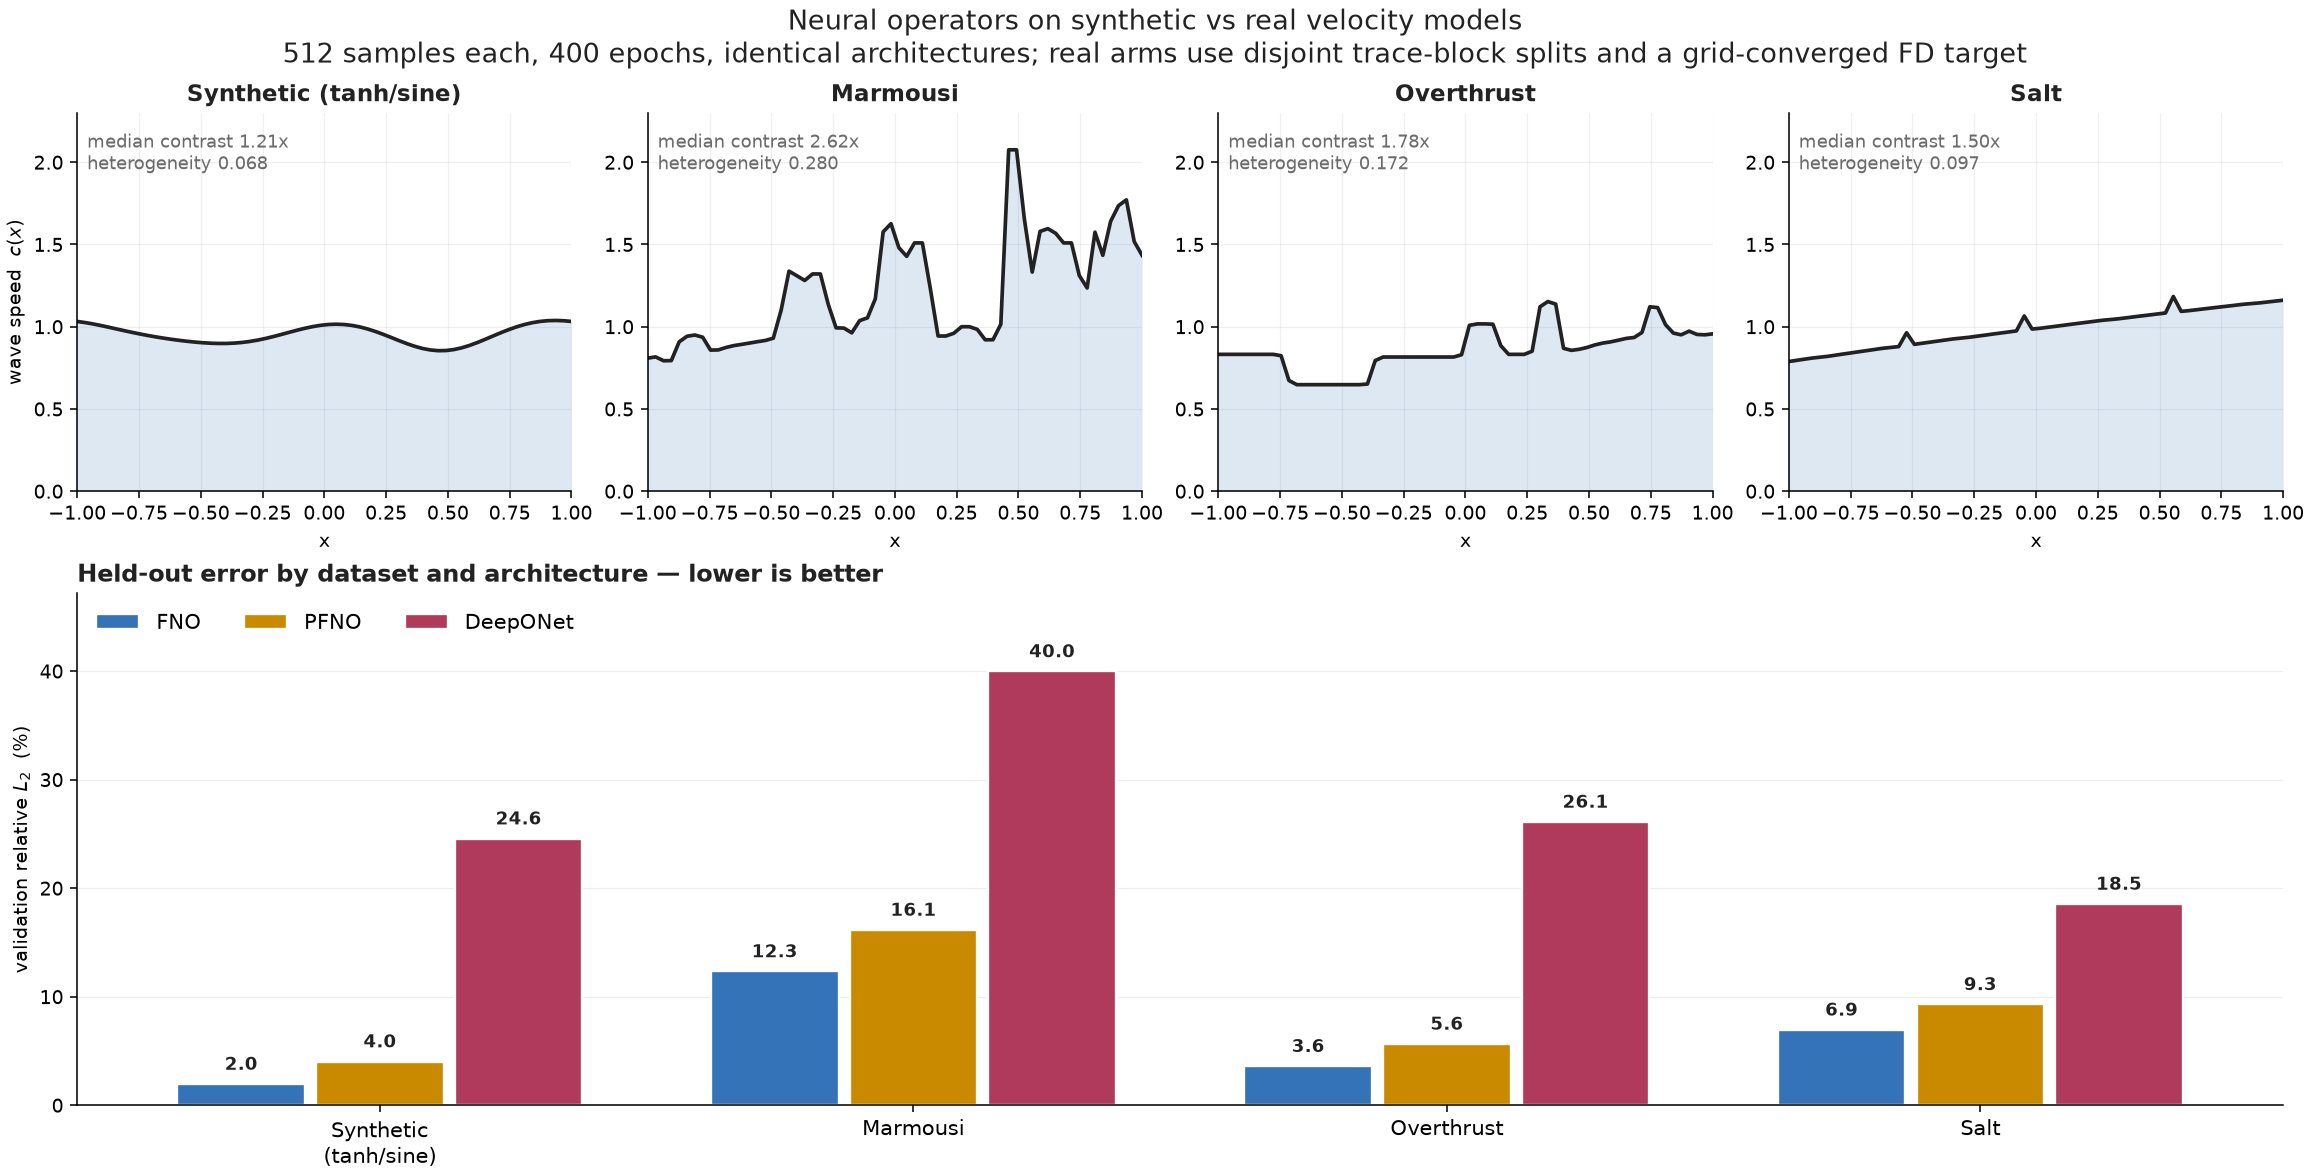
\includegraphics[width=\textwidth]{figures/real_models_comparison.png}
\caption{Held-out error by dataset and architecture. The ranking
FNO $<$ PFNO $<$ DeepONet holds on every arm.}
\end{figure}

\textbf{The architectural ranking survives on real geology} --- FNO $<$ PFNO $<$
DeepONet on every arm without exception, which is the main thing this section
was run to check. But the margins compress: FNO beats PFNO by $2.1\times$ on
synthetic data and only $1.3\times$ on Marmousi. And difficulty tracks
\textbf{heterogeneity, not contrast}. Marmousi and Overthrust actually get
\emph{easier} as $V_{p,\max}/V_{p,\min}$ rises, while Salt reverses completely,
because its high-contrast columns are exactly the ones intersecting a salt
body --- one sharp isolated reflector, which is a different and harder problem
than a wide velocity range.

\subsection{Visualization}

Twenty animations in \texttt{simulations/} (4 synthetic, 9 real, 4 forced, 3
superseded), each a $2\times4$ panel: the velocity model and three line-plot
comparisons on top, the FD reference field and three predicted fields below, all
on a shared colour scale. Three defects in the original figure were fixed,
because they mattered for interpretability independent of model quality:

\begin{enumerate}[leftmargin=*,itemsep=3pt]
\item \textbf{The reference is now shown.} The original compared the three
predictions against each other only --- actively misleading when models are
undertrained, since a near-zero field looks smooth and plausible.
\item \textbf{The colour scale comes from the propagating wave} (98th percentile
of $|u|$), not the global maximum. The $t=0$ pulse is about $1.8\times$ taller
than anything after it, so scaling to it spent half the colormap on a single
frame.
\item \textbf{The palette was re-stepped} for colour-vision separability. The
original blue/teal pair sat at $\Delta E=14.0$, below the legibility floor; the
worst adjacent pair is now $\Delta E=16.0$ under protanopia.
\end{enumerate}

Rendering is deliberately split from training: the training script writes no
plots, so the GPU host needs no matplotlib.

%==============================================================
\section{What the whole thing found}

\begin{enumerate}[leftmargin=*,itemsep=4pt]
\item \textbf{Operator learning has a hard data threshold.} Sixteen samples is
not a small dataset for this problem; it is below the point where anything is
learnable. A few hundred is the threshold, and generating them costs seconds.
\item \textbf{A near-zero prediction is the default failure}, and it looks
plausible. Every metric here is calibrated so that zero scores $\approx100\%$,
and every surprising result is checked against an amplitude-ratio control.
\item \textbf{The architectural ranking is stable and structural.} FNO $<$ PFNO
$<$ DeepONet on every material family, every real geological arm, forced and
unforced. It follows from what each architecture can represent: a joint $(x,t)$
spectrum, a per-frequency factorization, and a rank-$p$ separable expansion.
\item \textbf{Physics losses help a model that already fits, and hurt one that
does not.} FNO improves monotonically to $\lambda=10$; DeepONet is pushed
further toward the trivial solution that satisfies every homogeneous constraint
exactly.
\item \textbf{Residual diagnostics are not standalone evidence.} The worst model
had the best boundary residual.
\item \textbf{The reference solution is part of the experiment.} An unconverged
target left one architecture's headline number ten points too good.
\item \textbf{Difficulty is about sharp isolated reflectors, not velocity
range.} $V_{p,\max}/V_{p,\min}$ predicts the wrong sign on two of the three real
models.
\end{enumerate}

%==============================================================
\section{Repository map}

\paragraph{Code.}
\begin{center}
\small
\begin{tabular}{@{}>{\raggedright\arraybackslash}p{5.4cm}>{\raggedright\arraybackslash}p{9.7cm}@{}}
\toprule
\textbf{Path} & \textbf{Role}\\
\midrule
\texttt{wave/fd\_solver.py}        & leapfrog FD reference (conservative form, Mur ABC)\\
\texttt{wave/wave\_problem.py}     & torch-free problem definition: IC, material sampler, channel layout\\
\texttt{wave/materials.py}, \texttt{problem\_data.py} & Homogeneous / TwoLayer / MultiLayer $+$ JAX methods; ansatz, FD dispatch\\
\texttt{wave/run\_experiment.py}   & Arm A runner --- argparse, SLURM, backend switch, \texttt{MODEL\_CONFIGS} / \texttt{CONFIG}\\
\texttt{wave/sherlock.sh}          & the one cluster script (self-submitting, self-bootstrapping environment)\\
\texttt{wave/run\_fno\_baseline.py} & original FNO/CNN baseline; now re-exports \texttt{wave\_problem}\\
\texttt{wave/operator\_sim/}       & Arm B: dataset generation (synthetic / real / source), the three models, training, physics losses and metrics, rendering\\
\texttt{src/}                      & Arm A internals --- models, optimizers, training loops, losses, PyTorch and JAX\\
\texttt{kaggle/run\_fno\_t4.py}    & T4 preset launcher (smoke / medium / full)\\
\bottomrule
\end{tabular}
\end{center}

\paragraph{Data and results.}
\begin{center}
\small
\begin{tabular}{@{}>{\raggedright\arraybackslash}p{5.4cm}>{\raggedright\arraybackslash}p{9.7cm}@{}}
\toprule
\textbf{Path} & \textbf{Contents}\\
\midrule
\texttt{operator\_data/*.npz} & five datasets, $512\times5\times64\times64$ in / $512\times1\times64\times64$ out ($\sim$8.5 MB each): synthetic \texttt{refine=1}, synthetic \texttt{refine=8}, Marmousi, Overthrust, Salt, plus the forced arm at $64\times80$\\
\texttt{operator\_data/raw/}  & raw velocity models ($\sim$700 MB, gitignored)\\
\texttt{server\_outputs/}     & unforced synthetic run: predictions, summary, per-epoch histories, log\\
\texttt{server\_outputs\_real/} & the four real-model arms (\texttt{synthetic\_r8}, \texttt{marmousi}, \texttt{overthrust}, \texttt{salt})\\
\texttt{server\_outputs\_source/}, \texttt{server\_outputs\_pinn/} & forced arm, supervised and physics-informed (with \texttt{lambda\_sweep.json})\\
\texttt{simulations/}         & 20 GIFs --- synthetic, \texttt{real/}, \texttt{source\_term/}, \texttt{superseded\_undertrained/}\\
\texttt{fno\_t4\_\{smoke,medium,full\}/}, \texttt{operator\_results\_*}, \texttt{kaggle\_outputs/} & earlier baseline runs that bracket the data threshold\\
\texttt{final/}               & the earlier standalone project: checkpoints, exp1--3 results, numerical-methods comparison\\
\bottomrule
\end{tabular}
\end{center}

Model checkpoints (\texttt{FNO\_state.pt} alone is 59 MB) stayed on the training
host and were not copied back; predictions and summaries were, which is
everything the renderer and the analysis need.

\paragraph{Writing and reference material.}
\begin{center}
\small
\begin{tabular}{@{}>{\raggedright\arraybackslash}p{5.4cm}>{\raggedright\arraybackslash}p{9.7cm}@{}}
\toprule
\textbf{Path} & \textbf{Contents}\\
\midrule
\texttt{docs/operator\_simulations.*} & the full Arm B write-up (17 sections), Markdown $+$ \LaTeX{} $+$ PDF, with 11 figures\\
\texttt{notebooks/}      & end-to-end FNO/DeepONet/PFNO notebook (\texttt{QUICK\_RUN} toggle; uses pretrained predictions when present)\\
\texttt{ppt/}            & \texttt{FNO\_Technical\_Reference} (\LaTeX{} $+$ PDF), KAN guide, experiments deck, and \texttt{diagrams/} --- TikZ sources for spectral convolution, FNO2d, the Fourier block, ansatz anatomy, the data pipeline and architecture evolution\\
\texttt{presentations/}, \texttt{outputs/} & neural-operator architecture decks and the FNO explainer, several revisions\\
\texttt{videos/}         & two rendered FNO explainer videos\\
\texttt{papers/}         & $\sim$30 reference PDFs and a BibTeX file, with a curated seven-paper \texttt{FNO\_reading\_order/}\\
\texttt{fno paper/}      & the three papers the Arm B implementations follow\\
\bottomrule
\end{tabular}
\end{center}

%==============================================================
\section{Status and honest limits}

\paragraph{Done and measured.} The entire operator arm --- four material
regimes, forced and unforced, supervised and physics-informed, with converged
targets, spatially disjoint splits, calibrated metrics, animations, and a full
write-up.

\paragraph{Built but not reported here.} The 528-run PINN/KAN sweep. The code,
both backends, all seven architectures, SOAP / RBA / causal weighting / GradNorm
and the cluster harness are complete; the results live on cluster scratch rather
than in the repository, and no cross-architecture comparison has been written up
from them.

\paragraph{Limits to keep in view when reading Arm B's numbers.}
\begin{itemize}[leftmargin=*,itemsep=3pt]
\item \textbf{One seed, one split, no error bars.} Tenths of a percent between
configurations mean nothing; the order-of-magnitude gaps between architectures
do.
\item \textbf{Fixed initial condition} ($\sigma_g=0.1$, $x_0=0$) --- the unforced
arm learns a velocity-model $\to$ wavefield map, not a general initial-condition
$\to$ wavefield map.
\item \textbf{Fixed $64\times64$ grid.} FNO and PFNO are in principle
discretization-invariant; zero-shot super-resolution was never tested.
\item \textbf{In-distribution evaluation only.} No arm is evaluated on a
\emph{different} arm --- nothing trains on Marmousi and tests on Salt, which is
the transfer question a practitioner would actually ask. Transfer to Arm A's
canonical materials is also untested.
\item \textbf{``Real'' means published benchmark model, not measurement.}
Marmousi and Overthrust are themselves synthetic constructions, geologically
realistic but not logged rock; the wave field is FD-simulated in every arm. Only
Marmousi ships a density model.
\item \textbf{Parameters are not matched.} FNO has 7.4 M against DeepONet's
0.89 M and PFNO's 1.2 M, so some of FNO's advantage is capacity; a
parameter-matched comparison has not been run. Note also that
\texttt{train\_operators.py} defaults to a smaller DeepONet
(\texttt{--don-latent 192 --don-hidden 384}) than the $256/512$ pair every
DeepONet number here uses --- re-running without those flags silently produces a
smaller, non-comparable model.
\item \textbf{These are readable reimplementations}, sized to train in minutes,
not faithful reproductions of the Li et al.\ or Lu et al.\ configurations.
\end{itemize}

\paragraph{Version-control state.} Most of the work described in Section 4 ---
\texttt{wave/operator\_sim/}, \texttt{docs/}, \texttt{notebooks/},
\texttt{simulations/}, all \texttt{server\_outputs*} directories, and the
\texttt{ppt/} technical reference and diagrams --- is currently
\textbf{untracked}. Only the FNO baseline and the Kaggle runner have been
committed.

\end{document}
